\setcounter {section} {3}
\setcounter{ex}{0}
\section{Phương trình mũ -- Bất phương trình mũ}
\subsection{Kiến thức cần nhớ}
\begin{khung}
	\subsubsection{Công thức nghiệm của phương trình mũ}
	\begin{itemize}
		\item Dạng \fbox{$a^x=b$} (1), với $a>0$ và $a \ne 1$.
		\item  Về mặt đồ thị, nghiệm của (1) là hoành độ giao điểm của đồ thị $y=a^x$ với đường thẳng $y=b$ (nằm ngang). 
		\immini{Từ hình vẽ, ta có các kết quả sau:
			
			\begin{listEX}[1]
				\item  $b>0$ (1) có nghiệm duy nhất $x=\log_ab$.
				\item  $b\le 0$ (1) vô nghiệm.
			\end{listEX}
			
			
		}{	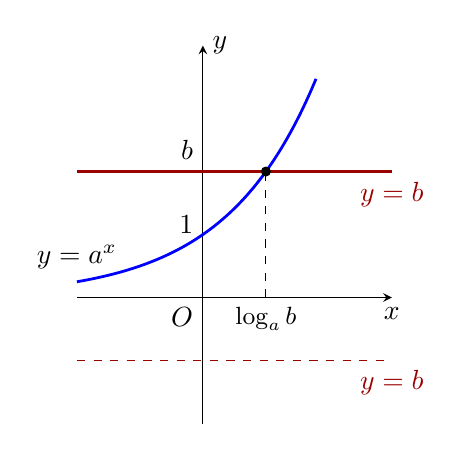
\begin{tikzpicture}[smooth,samples=300,scale=0.8,>=stealth]
				\draw[->] (-2,0)--(3,0) node[below]{$x$};
				\draw[->] (0,-2)--(0,4) node[right]{$y$};
				\draw (0,0) node[below left]{$O$};
				\draw[line width=1pt,color=blue,domain=-2:1.8] plot(\x,{2^(\x)});
				\draw[color=red!60!black,line width=1pt] (-2,2)--(3,2) node[below]{$y=b$};
				\draw[dashed,color=red!60!black] (-2,-1)--(3,-1) node[below]{$y=b$};
				\draw[dashed] (1,0)node[below]{\small$\log_ab$}--(1,2);
				\draw[fill=black](1,2) circle(2pt);
				\node[above] at (-2,0.3) {$y=a^x$};
				\node[left] at (0,2.35) {$b$};
				\node[left] at (0,1.15) {$1$};
		\end{tikzpicture}}
		
		\item \textbf{Tóm lại:} Với $a>0$ và $a \ne 1$, $b>0$, ta có các công thức sau đây: 
		\begin{listEX}[2]
			\item  $a^{f(x)}=b \Leftrightarrow f(x)=\log_ab$.
			\item  $a^{f(x)}=a^{g(x)} \Leftrightarrow f(x)=g(x)$.
		\end{listEX}
	\end{itemize}
	\subsubsection{Công thức nghiệm của bất phương trình mũ}
	Minh họa dạng \fbox{$a^x>b$}, với $a>0$ và $a \ne 1$.\\
	\hspace*{1cm}
	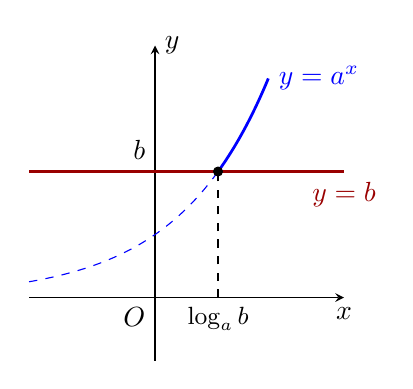
\begin{tikzpicture}[smooth,samples=300,scale=0.8,>=stealth]
		\draw[->] (-2,0)--(3,0) node[below]{$x$};
		\draw[->] (0,-1)--(0,4) node[right]{$y$};
		\draw (0,0) node[below left]{$O$};
		\draw[dashed,color=blue,domain=-2:1] plot(\x,{2^(\x)});
		\draw[line width=1pt,color=blue,domain=1:1.8] plot(\x,{2^(\x)})node[right]{$y=a^x$};
		\draw[color=red!60!black,line width=1pt] (-2,2)--(3,2) node[below]{$y=b$};
		\draw[dashed] (1,0)node[below]{\small$\log_ab$}--(1,2);
		\draw[fill=black](1,2) circle(2pt);
		\node[left] at (0,2.35) {$b$};
	\end{tikzpicture}
	\hspace{3cm}
	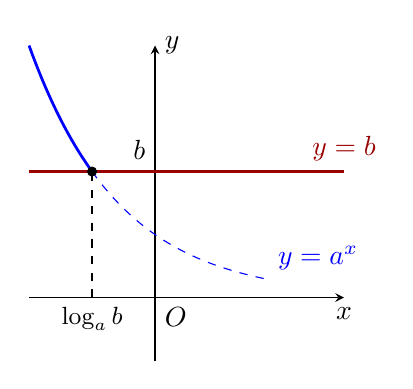
\begin{tikzpicture}[smooth,samples=300,scale=0.8,>=stealth]
		\draw[->] (-2,0)--(3,0) node[below]{$x$};
		\draw[->] (0,-1)--(0,4) node[right]{$y$};
		\draw (0,0) node[below right]{$O$};
		\draw[dashed,color=blue,domain=-1:1.8] plot(\x,{0.5^(\x)})node[above right]{$y=a^x$};
		\draw[line width=1pt,color=blue,domain=-2:-1] plot(\x,{0.5^(\x)});
		\draw[color=red!60!black,line width=1pt] (-2,2)--(3,2) node[above]{$y=b$};
		\draw[dashed] (-1,0)node[below]{\small$\log_ab$}--(-1,2);
		\draw[fill=black](-1,2) circle(2pt);
		\node[left] at (0,2.35) {$b$};
	\end{tikzpicture}
	\begin{itemize}
		\item [$\bullet$] Nếu $b \le 0$ thì tập nghiệm của bất phương trình là $\mathbb{R}$.
		\item [$\bullet$] Nếu $b>0$, ta có hai trường hợp:
		\begin{listEX}[1]
			\item Với $a>1$ thì $a^x>b \Leftrightarrow x>\log_ab$ (Hình 1).
			\item  Với $0<a<1$ thì $a^x>b \Leftrightarrow x<\log_ab$ (Hình 2).
		\end{listEX}
	\end{itemize}
	
\end{khung}
\subsection{Bài tập mẫu}
%\Opensolutionfile{ans}[ans/ANS-DANG-1]
\begin{khung}
	\begin{vd}%[2D2Y6-2]%[ĐỀ MH BGD 2022-2023]%[Nguyễn Huynh]
		Tập nghiệm của bất phương trình $2^{x+1}<4$ là
		\choice
		{$(-\infty; 1]$}
		{$(1; +\infty)$}
		{$[1; +\infty)$}
		{\True $(-\infty; 1)$}
		\loigiai{
			Ta có	$2^{x+1}<4\Leftrightarrow 2^{x+1}<2^2\Leftrightarrow x+1<2\Leftrightarrow x<1$.\\
			Tập nghiệm của bất phương trình là $(-\infty; 1)$.
		}
	\end{vd}
\end{khung}
\subsection{Bài tập tương tự và phát triển}
\Opensolutionfile{ans}[ans/ANS-DANG-4]
\begin{ex}%[Nguyễn Huynh]%[2D2B5-2] 
	Phương trình ${\left( \dfrac{1}{3} \right)}^{x^2-2x-3}=3^{x+1}$ có bao nhiêu nghiệm?
	\choice
	{\True  $2$}
	{ $1$}
	{ $0$}
	{ $3$}
	\loigiai{Ta có ${\left( \dfrac{1}{3} \right)}^{x^2-2x-3}=3^{x+1}\Leftrightarrow {\left( \dfrac{1}{3} \right)}^{x^2-2x-3}={\left( \dfrac{1}{3} \right)}^{-x-1}\Leftrightarrow x^2-2x-3=-x-1\Leftrightarrow \hoac{
			& x=-1 \\
			& x=2.}$	\\Vậy phương trình có 2 nghiệm $x=-1;x=2.$}
\end{ex}

\begin{ex}%[2D2B5-2]%[Nguyễn Huynh] 
	Nghiệm của phương trình $4^{x+1}=8^{2x-3}$ là
	\choice
	{ $x=\dfrac{11}{2}$}
	{ $x=\dfrac{11}{3}$}
	{\True  $x=\dfrac{11}{4}$}
	{ $x=\dfrac{11}{5}$}
	\loigiai{
		Ta có $4^{x+1}=8^{2x-3}\Leftrightarrow 2^{2x+2}=2^{3\left( 2x-3 \right)}\Leftrightarrow 2x+2=6x-9\Leftrightarrow x=\dfrac{11}{4}$.}
\end{ex}

\begin{ex}%[2D2B5-2]%[Nguyễn Huynh] 
	Tìm tập nghiệm của phương trình $4^{x^2}=2^{x+1}$.
	\choice
	{ $S=\left\{ 0;1 \right\}$}
	{\True  $S=\left\{ -\dfrac{1}{2};1 \right\}$}
	{ $S=\left\{ \dfrac{1-\sqrt{5}}{2};\dfrac{1+\sqrt{5}}{2} \right\}$}
	{ $S=\left\{ -1;\dfrac{1}{2} \right\}$}
	\loigiai{	Ta có $4^{x^2}=2^{x+1}\Leftrightarrow 2^{2x^2}={2^{x+1}}\Leftrightarrow 2x^2=x+1\Leftrightarrow \hoac{&
			x=1  \\&
			x=-\dfrac{1}{2}.}$\\
		Vậy $S=\left\{ -\dfrac{1}{2};1 \right\}$.}
\end{ex}

\begin{ex}%[2D2Y5-2]%[Nguyễn Huynh] 
	Nghiệm của phương trình $3^{2x+1}=27$ là
	\choice
	{ $x=2$}
	{\True  $x=1$}
	{ $x=\dfrac{1}{2}$}
	{ $x=\dfrac{3}{2}$}
	\loigiai{
		Ta có $3^{2x+1}=27$ $\Leftrightarrow 3^{2x+1}=3^3$ $\Leftrightarrow 2x+1=3\Leftrightarrow x=1$.}
\end{ex}

\begin{ex}%[2D2B6-2]%[Nguyễn Huynh]
	Tập nghiệm của bất phương trình $3^{x+2}<9^{2x+7}$.
	\choice
	{ $\left( -5;+\infty  \right)$}
	{ $\left( -\infty ;-5 \right)$}
	{\True  $\left( -4;+\infty  \right)$}
	{ $\left( -\infty ;-4 \right)$}
	\loigiai{
		Ta có $3^{x+2}<9^{2x+7}\Leftrightarrow 3^{x+2}<3^{2\left( 2x+7 \right)}\Leftrightarrow x+2<4x+14\Leftrightarrow x>-4$.\\
		Vậy $S=\left( -4;+\infty  \right)$.}
\end{ex}

\begin{ex}%[2D2Y6-2]%[Nguyễn Huynh]
	Tập nghiệm của bất phương trình $2^{100x}\ge 4^{200}$ là
	\choice
	{ $\left( -\infty ;4 \right]$}
	{\True  $\left[ 4;+\infty  \right)$}
	{ $\left[ 2;+\infty  \right)$}
	{ $\left( 4;+\infty  \right)$}
	\loigiai{
		Ta có	$2^{100x}\ge 4^{200}\Leftrightarrow 2^{100x}\ge 2^{400}\Leftrightarrow 100x\ge 400\Leftrightarrow x\ge 4$. 
		Vậy $S=\left[ 4;+\infty  \right)$.}
\end{ex}

\begin{ex}%[2D2B5-2]%[Nguyễn Huynh] 
	Nghiệm của phương trình $5^{x-4}=\left( \dfrac{1}{25} \right)^{3x-1}$ là
	\choice
	{\True  $x=\dfrac{6}{7}$}
	{ $x=\dfrac{1}{3}$}
	{ $x=1$}
	{ $x=\dfrac{7}{6}$}
	\loigiai{
		Ta có $5^{x-4}=\left( \dfrac{1}{25} \right)^{3x-1}\Leftrightarrow 5^{x-4}=5^{-6x+2}\Leftrightarrow x-4=-6x+2\Leftrightarrow x=\dfrac{6}{7}$.}
\end{ex}

\begin{ex}%[2D2B6-2]%[Nguyễn Huynh] 
	Bất phương trình $3^{x^2+1}>3^{2x+1}$ có tập nghiệm là
	\choice
	{ $S=\left( -2;0 \right)$}
	{ $S=\left( 0;2 \right)$}
	{ $S=\mathbb{R}$}
	{\True  $S=\left( -\infty ;0 \right)\cup \left( 2;+\infty  \right)$}
	\loigiai{
		Ta có $3^{x^2+1}>3^{2x+1}\Leftrightarrow x^2+1>2x+1\Leftrightarrow x^2-2x>0\Leftrightarrow \hoac{
			& x>2 \\
			& x<0.}$ \\
		Do đó $S=\left( -\infty ;0 \right)\cup \left( 2;+\infty  \right)$.}
\end{ex}

\begin{ex}%[2D2Y5-2]%[Nguyễn Huynh] 
	Nghiệm của phương trình $5^{2x+1}=125$ là
	\choice
	{\True  $x=1$}
	{ $x=3$}
	{ $x=2$}
	{ $x=4$}
	\loigiai{
		Ta có $5^{2x+1}=5^3$
		$\Leftrightarrow 2x+1=3$
		$\Leftrightarrow x=1$.\\
		Vậy nghiệm của phương trình là $x=1$.}
\end{ex}

\begin{ex}%[2D2Y5-2]%[Nguyễn Huynh] 
	Tập nghiệm của phương trình $2^{x^2-3x}=\dfrac{1}{4}$ là
	\choice
	{ $S=\varnothing $}
	{\True  $S=\left\{ 1;2 \right\}$}
	{ $S=\left\{ 0 \right\}$}
	{ $S=\left\{ 1 \right\}$}
	\loigiai{
		Ta có $2^{x^2-3x}=\dfrac{1}{4}\Leftrightarrow 2^{x^2-3x}=2^{-2}\Leftrightarrow x^2-3x=-2\Leftrightarrow x^2-3x+2=0\Leftrightarrow\hoac{
			& x=1 \\
			& x=2. }$\\
		Vậy tập nghiệm của phương trình là $S=\left\{ 1;2 \right\}$.}
\end{ex}

\begin{ex}%[2D2B6-2]%[Nguyễn Huynh]
	Bất phương trình ${\left( \dfrac{1}{2} \right)}^{x^2-2x}>\dfrac{1}{8}$ có tập nghiệm là $\left( a;b \right)$. Khi đó giá trị của $b-a$ là
	\choice
	{ $-2$}
	{ $-4$}
	{ $2$}
	{\True  $4$}
	\loigiai{
		${\left( \dfrac{1}{2} \right)}^{x^2-2x}>\dfrac{1}{8}\Leftrightarrow x^2-2x<{\log }_{\dfrac{1}{2}}\left( \dfrac{1}{8} \right)\Leftrightarrow x^2-2x-3<0\Leftrightarrow -1<x<3$.\\
		Tập nghiệm của bất phương trình là $\left( -1;3 \right)$.\\
		Khi đó $a=-1$ và $b=3$.
		Vậy $b-a=4$.}
\end{ex}

\begin{ex}%[2D2B5-2]%[Nguyễn Huynh] 
	Giải phương trình $\left( \dfrac{1}{25} \right)^{x-1}={125}^{2x}$.
	\choice
	{ $x=-\dfrac{1}{8}$}
	{\True  $x=\dfrac{1}{4}$}
	{ $x=4$}
	{ $x=-\dfrac{1}{4}$}
	\loigiai{
		Ta có $\left( \dfrac{1}{25} \right)^{x-1}={125}^{2x}={125}^{2x}\Leftrightarrow 5^{-2x+2}=5^{6x}\Leftrightarrow $ $-2x+2=6x\Leftrightarrow x=\dfrac{1}{4}$.}
\end{ex}

\begin{ex}%[2D2B5-2]%[Nguyễn Huynh] 
	Nghiệm của phương trình $\left( \sqrt{2} \right)^{2x+1}=\left( \dfrac{1}{2} \right)^{3x}$là
	\choice
	{ $x=-\dfrac{1}{2}$}
	{ $x=-\dfrac{1}{5}$}
	{ $x=\dfrac{1}{4}$}
	{\True  $x=-\dfrac{1}{8}$}
	\loigiai{
		Ta có $\left( \sqrt{2} \right)^{2x+1}=\left( \dfrac{1}{2} \right)^{3x}\Leftrightarrow 2^{\frac{1}{2}\left( 2x+1 \right)}=2^{-3x}\Leftrightarrow x+\dfrac{1}{2}=-3x\Leftrightarrow x=-\dfrac{1}{8}$.}
\end{ex}

\begin{ex}%[2D2Y6-2]%[Nguyễn Huynh] 
	Tập nghiệm của bất phương trình $2^{2x}<2^{x+6}$ là
	\choice
	{\True  $\left( -\infty ;6 \right)$}
	{ $\left( 0;64 \right)$}
	{ $\left( 6;+\infty  \right)$}
	{ $\left( 0;6 \right)$}
	\loigiai{
		Ta có $2^{2x}<2^{x+6}\Leftrightarrow 2x<x+6\Leftrightarrow x<6$.\\
		Vậy tập nghiệm của bất phương trình là $S=\left( -\infty ;6 \right)$.}
\end{ex}

\begin{ex}%[2D2B6-2]%[Nguyễn Huynh] 
	Tìm tập nghiệm của bất phương trình $2^{x^2-5x+4}\le 1$.
	\choice
	{\True  $\left[ 1;4 \right]$}
	{ $\left( -\infty ;1 \right]\cup \left[ 4;+\infty  \right)$}
	{ $\left( -\infty ;1 \right]$}
	{ $\left[ 4;+\infty  \right)$}
	\loigiai{
		Ta có $2^{x^2-5x+4}\le 1\Leftrightarrow 2^{x^2-5x+4}\le 2^0\Leftrightarrow x^2-5x+4\le 0\Leftrightarrow 1\le x\le 4$.\\
		Vậy $S=\left[ 1;4 \right].$}
\end{ex}

\begin{ex}%[2D2Y5-2]%[Nguyễn Huynh]
	Nghiệm của phương trình $2^{x+2}=32$ là
	\choice
	{ $x=7$}
	{ $x=8$}
	{\True  $x=3$}
	{ $x=4$}
	\loigiai{
		Ta có $2^{x+2}=32\Leftrightarrow 2^{x+2}=2^5\Leftrightarrow x+2=5\Leftrightarrow x=3$.\\
		Vậy phương trình có nghiệm $x=3$.}
\end{ex}

\begin{ex}%[2D2Y5-2]%[Nguyễn Huynh] 
	Nghiệm của phương trình $5^{x-4}=\left( \dfrac{1}{25} \right)^{3x-1}$là
	\choice
	{ $x=\dfrac{7}{6}$}
	{\True  $x=\dfrac{6}{7}$}
	{ $x=\dfrac{1}{3}$}
	{ $x=1$}
	\loigiai{
		Ta có $5^{x-4}=\left( \dfrac{1}{25} \right)^{3x-1}\Leftrightarrow5^{x-4}=5^{-6x+2}\Leftrightarrow x-4=-6x+2\Leftrightarrow x=\dfrac{6}{7}$.}
\end{ex}



\begin{ex}%[2D2Y5-2]%[Nguyễn Huynh]
	Tập nghiệm của phương trình ${2^{x^2+x+1}}=8$ là
	\choice
	{ $\left\{ 1 \right\}$}
	{\True  $\left\{ -2\text{ };\text{ }1 \right\}$}
	{ $\left\{ -2 \right\}$}
	{ $\left\{ 1\text{ };\text{ }2 \right\}$}
	\loigiai{
		Ta có ${2^{x^2+x+1}}=8\Leftrightarrow {2^{x^2+x+1}}=2^3\Leftrightarrow x^2+x+1=3\Leftrightarrow x^2+x-2=0\Leftrightarrow \hoac{
			& x=1 \\
			& x=-2.}$\\
		Vậy tập nghiệm của phương trình là $S=\left\{ -2; 1 \right\}$.}
\end{ex}

\begin{ex}%[2D2Y5-2]%[Nguyễn Huynh]
	Nghiệm của phương trình ${3^{2x-1}}=27$
	\choice
	{ $x=1$}
	{\True  $x=2$}
	{ $x=3$}
	{ $x=4$}
	\loigiai{
		Ta có ${3^{2x-1}}=27\Leftrightarrow {3^{2x-1}}=3^3\Leftrightarrow 2x-1=3\Leftrightarrow 2x=4\Leftrightarrow x=2$.}
\end{ex}

\begin{ex}%[2D2B5-2]%[Nguyễn Huynh]
	Tập nghiệm của phương trình ${2^{x^2-3x}}=\dfrac{1}{4}$ là
	\choice
	{ $S=\left\{ 0 \right\}$}
	{ $S=\left\{ 1 \right\}$}
	{ $S=\varnothing $}
	{\True  $S=\left\{ 1;2 \right\}$}
	\loigiai{
		Ta có ${2^{x^2-3x}}=\dfrac{1}{4}\Leftrightarrow {2^{x^2-3x}}={2^{-2}}\Leftrightarrow x^2-3x=-2\Leftrightarrow x^2-3x+2=0\Leftrightarrow\hoac{
			& x=1 \\
			& x=2.}$\\
		Vậy tập nghiệm của phương trình là $S=\left\{ 1;2 \right\}$.}
\end{ex}

\begin{ex}%[2D2Y5-2]%[Nguyễn Huynh]
	Số nghiệm của phương trình $3^x={\left( \dfrac{1}{3} \right)}^x$ là
	\choice
	{ $2$}
	{ $3$}
	{ $0$}
	{\True  $1$}
	\loigiai{
		Ta có $3^x={\left( \dfrac{1}{3} \right)}^x\Leftrightarrow 3^x=3^{-x}\Leftrightarrow x=-x\Leftrightarrow x=0.$}
\end{ex}

\begin{ex}%[2D2Y6-2]%[Nguyễn Huynh]
	Tập nghiệm của bất phương trình $2^{x+2}<\left( \dfrac{1}{4} \right)^x$ là
	\choice
	{ $\left( -\infty ;0 \right)$}
	{ $\left( -\dfrac{2}{3};+\infty  \right)$}
	{ $\left( 0;+\infty  \right)\setminus \left\{ 1 \right\}$}
	{\True  $\left( -\infty ;-\dfrac{2}{3} \right)$}
	\loigiai{
		Ta có $2^{x+2}<\left( \dfrac{1}{4} \right)^x\Leftrightarrow 2^{x+2}<2^{-2x}\Leftrightarrow x+2<-2x\Leftrightarrow x<-\dfrac{2}{3}$.\\
		Vậy tập nghiệm của bất phương trình là $\left( -\infty ;-\dfrac{2}{3} \right).$}
\end{ex}


\begin{ex}%[2D2B6-2]%[Nguyễn Huynh]
	Tập nghiệm bất phương trình $2^{x^2-3x}<16$ là
	\choice
	{ $\left( 4;+\infty  \right)$}
	{\True  $\left( -1;4 \right)$}
	{ $\left( -\infty ;-1 \right)\cup \left( 4;+\infty  \right)$}
	{ $\left( -\infty ;-1 \right)$}
	\loigiai{
		Ta có	$2^{x^2-3x}<16\Leftrightarrow 2^{x^2-3x}<2^4\Leftrightarrow x^2-3x<4\Leftrightarrow -1<x<4$.
	}
\end{ex}
\Closesolutionfile{ans}
%======================
\subsection{Bảng đáp án}
\inputansbox{8}{ans/ANS-DANG-4}